%% !TEX TS-programm = lualatex
% !BIB program = biber
% !TEX spellcheck = de_DE

\documentclass[greek,ngerman,parskip=half,
%draft%zeigt Formatierung an
]{scrbook}
%\PassOptionsToPackage{draft}{graphicx}%beschränkt "draft" auf package graphicx


% !TEX root=../august-boeckh-hauptdokument.tex

\usepackage{babel}

\usepackage{graphicx}
\graphicspath{{figures/}}%relativer Pfad zu den Bildern
\usepackage{caption}
\usepackage{subcaption}%für Bilder nebeneinander

\usepackage[
%content={Abbildung ausgeblendet, damit ich schneller kompilieren kann.},%Platzhaltertext
%filename,%Pfad anzeigen
size=normalsize,%Größe der Platzhalter
position=center,%Position des Platzhalters
noframe,%kein Rahmen
]{draftfigure}%modifizieren von ausgeblendeten Abbildungen

\usepackage{multicol}%mehrspaltiger Text

\widowpenalty=10000 %vermeide Schusterjungen
\clubpenalty=10000 %vermeide Hurenkinder

\usepackage{libertine}
\usepackage{xspace}
\usepackage[dvipsnames]{xcolor}

\usepackage{imakeidx}
\makeindex[
name=per,%Dies ist ein Personenindex
title = {Index antiker Personen},
columns=1,
options={-s style/index-style.tex},
]

\makeindex[
name=ant,
title = {Index antiker Texte},
columns=3,
options={-s style/index-style.tex},
]

\indexsetup{%
level=\addsec,%entspricht \section*
firstpagestyle=scrheadings, %normale Seitenformatierung
headers={\indexname}{\indexname}, %Kolumnentitel auf beiden Seiten
}

\usepackage[
series={},
nocritical,
noend,
noeledsec,
nofamiliar,
noledgroup
]{reledmac}%am besten für Übersetzungen
\usepackage{reledpar}

\usepackage{tabularx}%für Tabellen
\usepackage{booktabs}%für schöne Tabellen
\usepackage{tablefootnote}%für Fußnoten in Tabellen

\usepackage[headsepline=.5pt]
{scrlayer-scrpage}

\usepackage[singlelinecheck=false]{caption}

\usepackage{chngcntr}%Änderung von Nummerierungen
\counterwithout{table}{chapter}

\usepackage{marginnote}%für Marginalspalten

\usepackage{datatool}
\DTLloaddb%
{archaeologen}%Interner Name der Datenbank
{data/archaeologen.csv}%Speicherort

\DTLloaddb%lade Datenbank
{kaiser}%interner Name
{data/kaiser.csv}%Speicherort der Datei


\usepackage[section=subsection,%Glossar direkt nach Bezugstext
nonumberlist,%keine Seitenzahl
nopostdot,%kein Punkt ans Ende
]{glossaries}%für Glossare
\makeglossaries

\usepackage{SIunits}

\DTLloaddb{fachstudenten}
{data/fachstudenten.csv}

\DTLloaddb{haeuser}
{data/haeuser.csv}

\usepackage{databar}%für Balkendiagramme
\usepackage{datapie}%für Tortendiagramme

\usepackage{etoolbox}%für kondizionale Operatoren
\newtoggle{hund}%Definiert Bedingung.
\newtoggle{nocopyright}

\newcommand\missingcopyright{
\iftoggle{nocopyright}
{\setkeys{Gin}{draft}%setzt Bild auf draft
\setkeys{draftfigure}{%
filename = true,
content = {Abbildung musste aufgrund fehlender Digitalrechte ausgeblendet werden.}}}
{}}
% !TEX root=../august-boeckh-hauptdokument.tex

\setkomafont{disposition}{\normalfont}%Überschriften normal
\setkomafont{chapter}{\Huge\scshape}%Kapitelüberschriften als Kapitälchen
\setkomafont{section}{\Large\itshape}

\addtokomafont{footnotenumber}{\footnotesize\normalfont\sffamily}%Änderung der Fußnotennummerierung (geht auch mit \setkomafont)
\setkomafont{pageheadfoot}{\sffamily}

\deffootnote%
{0.075cm}%Einrückung
{\normalparindent}%Paragraphenabsatz
{\makebox[\normalparindent][r]{\thefootnotemark\ }}
\newlength{\normalparindent}
\AtBeginDocument{\setlength{\normalparindent}{\parindent}}
%\setfootnoterule{0pt}

\makeatletter
\newcommand\BC{\,v.\,Chr\@ifnextchar.{}{.\relax\@\xspace}}
\newcommand\AD{\,n.\,Chr\@ifnextchar.{}{.\relax\@\xspace}}
\makeatother

\newcommand\Index[1]{\index[per]{#1}#1\xspace}
\newcommand\Indexmargin[1]{\index[per]{#1}\marginnote{#1}#1\xspace}

\newcommand\mysideref[1]{\marginnote{Abb. \ref{fig:#1}}}%Referenzen in der Marginalspalte

%Eigene Änderungen
% !TEX root=../august-boeckh-hauptdokument.tex

\iffalse%alles Nachfolgende wird ignoriert.
\newglossaryentry{Augustus}{name={\textbf{Augustus}},
	description={Augustus (Imperator Caesar Divi Filius Augustus),
		\newline *63\BC
		\newline gest. 14\AD
		\newline (27\BC -- 14\AD)},
	first={Augustus (27\protect\BC -- 14\protect\AD)}
}

\newglossaryentry{Mark Anton}{
	name={Mark Anton},
	description={Verräter},
	first={Mark Anton (der Verräter)}
}

\newglossaryentry{Kleopatra}{
	name={Kleopatra},%
	description={Kleopatra (Κλεοπάτρα Θεά Φιλοπάτωρ)
		\newline *69\BC
		\newline gest. 30\BC
		\newline aus dem Geschlecht der Ptolemäer, letzte der Pharaonen},%
	first={\textbf{Kleopatra}}
}
\fi%bis hierher wird ignoriert

\glssetexpandfield{name}
\glssetexpandfield{desc}
\glssetexpandfield{first}
\DTLforeach*{kaiser}%Datenbank aufrufen
{\kaiser=Kaiser,%
\name=Name,%
\geburt=Geburt,%
\geburtsort=Geburtsort,%
\tod=Tod,%
\sterbeort=Sterbeort,%
\reign=Regierungszeit,%
\shortreign=Regierungszeitkurz}%
{\newglossaryentry{\kaiser}%
{name={\textbf{\kaiser}},
description = {\kaiser
	\ifdefempty{\name}{}{\xspace(\name)};
\newline \geburt\xspace \ifdefempty{\geburtsort}{}{\xspace in \geburtsort}
\newline regierte\xspace\reign},
first = {\kaiser\ifdefempty{\shortreign}{}{\xspace\shortreign}}}}





\newtoggle{testdokument}
\newtoggle{finalpdf}
%\toggletrue{finalpdf}
%\toggletrue{testdokument}
\toggletrue{nocopyright}
\iftoggle{finalpdf}{
\togglefalse{testdokument}}%um sicherzugehen, dass nirgendwo anders der andere Toggle als true gesetzt ist.
{\iftoggle{testdokument}{}
{\includeonly{
	%content/mehrspaltiger-text,
	%content/tabellen,
	%content/glossar,
	%content/serienbriefe,
	%content/indexe,
	%content/wiederholende-info,
	%content/glossar,
	%content/serienbriefe
	%content/katalog
	%content/operatoren
	content/abbildungen}
}%false (testdokument)
}%false (finalpdf)

\begin{document}
\iftoggle{testdokument}{% !TEX root=../august-boeckh-hauptdokument.tex

Das ist das Testdokument.}
{% !TEX root=../august-boeckh-hauptdokument.tex

\begin{titlepage}
\hfill\includegraphics[width=.5\linewidth]{figures/hu-berlin}


%[[LOGO der HU]]
\vfill
\begin{center}
\Large
August Boeckh\par
\textit{Dissertation}
\end{center}
\vfill
Humboldt-Universität zu Berlin

August-Boeckh-Antikezentrum
\end{titlepage}
	


%----
% Titelseite
%----
\setcounter{tocdepth}{0}%Ebenen im Inhaltsverzeichnis
\tableofcontents


%---
% - Änderungsmöglichkeiten für das Aussehen des TOC?
% - Nur Kapitel in das Inhaltsverzeichnis?
%---

% !TEX root=../august-boeckh-hauptdokument.tex

\chapter{Mein mehrspaltiger Text}


%---
% Diesen Text bitte mehrspaltig setzen
%---
\begin{multicols}{2}[\section{Goethe – Werther}]

Eine wunderbare Heiterkeit hat meine ganze Seele eingenommen, gleich den süßen Frühlingsmorgen, die ich mit ganzem Herzen genieße. Ich bin allein und freue mich meines Lebens in dieser Gegend, die für solche Seelen geschaffen ist wie die meine. Ich bin so glücklich, mein Bester, so ganz in dem Gefühle von ruhigem Dasein versunken, daß meine Kunst darunter leidet. Ich könnte jetzt nicht zeichnen, nicht einen Strich, und bin nie ein größerer Maler gewesen als in diesen Augenblicken.\footnote{Komischer erster Absatz.}

Wenn das liebe Tal um mich dampft, und die hohe Sonne an der Oberfläche der undurchdringlichen Finsternis meines Waldes ruht, und nur einzelne Strahlen sich in das innere Heiligtum stehlen, ich dann im hohen Grase am fallenden Bache liege, und näher an der Erde tausend mannigfaltige Gräschen mir merkwürdig werden; wenn ich das Wimmeln der kleinen Welt zwischen Halmen, die unzähligen, unergründlichen Gestalten der Würmchen, der Mückchen näher an meinem Herzen fühle, und fühle die Gegenwart des Allmächtigen, der uns nach seinem Bilde schuf, das Wehen des Alliebenden,\footnote{Sehr schnulzig hier.} der uns in ewiger Wonne schwebend trägt und erhält; mein Freund!

Wenn's dann um meine Augen dämmert, und die Welt um mich her und der Himmel ganz in meiner Seele ruhn wie die Gestalt einer Geliebten - dann sehne ich mich oft und denke : ach könntest du das wieder ausdrücken, könntest du dem Papiere das einhauchen, was so voll, so warm in dir lebt, daß es würde der Spiegel deiner Seele, wie deine Seele ist der Spiegel des unendlichen Gottes! - mein Freund - aber ich gehe darüber zugrunde, ich erliege unter der Gewalt der Herrlichkeit dieser Erscheinungen.

Eine wunderbare Heiterkeit hat meine ganze Seele eingenommen, gleich den süßen Frühlingsmorgen, die ich mit ganzem Herzen genieße.\footnote{Ohje ohje, das ist ja mal ein Text, der es in sich hat und mich noch sehr beschäftigen wird, aber am Ende wird er mir vielleicht doch tatsächlich gefallen.} Ich bin allein und freue mich meines Lebens in dieser Gegend, die für solche Seelen geschaffen ist wie die meine. Ich bin so glücklich, mein Bester, so ganz in dem Gefühle von ruhigem Dasein versunken, daß meine Kunst darunter leidet. Ich könnte jetzt nicht zeichnen, nicht einen Strich, und bin nie ein größerer Maler gewesen als in diesen Augenblicken.

Wenn das liebe Tal um mich dampft, und die hohe Sonne an der Oberfläche der undurchdringlichen Finsternis meines Waldes ruht, und nur einzelne Strahlen sich in das innere Heiligtum stehlen, ich dann im hohen Grase am fallenden Bache liege, und näher an der Erde tausend mannigfaltige Gräschen mir merkwürdig werden; wenn ich das Wimmeln der kleinen Welt zwischen Halmen, die unzähligen, unergründlichen Gestalten der Würmchen…\footnote{Ein Würmchen, soso.}
\end{multicols}

 
%---
% Bitte griechisch links und deutsch rechts
%---
\section{Übersetzung „Griechisch / Deutsch“}

\begin{pairs}
\begin{Leftside}
\scriptsize
\beginnumbering
%\selectlanguage{greek}
\pstart
Μῆνιν ἄειδε θεὰ Πηληιάδεω Ἀχιλῆος\\ 
οὐλομένην, ἣ μυρί' Ἀχαιοῖς ἄλγε' ἔθηκε,\\ 
πολλὰς δ' ἰφθίμους ψυχὰς Ἄιδι προίαψεν\\ 
ἡρώων, αὐτοὺς δὲ ἑλώρια τεῦχε κύνεσσιν\\	
οἰωνοῖσί τε πᾶσι, Διὸς δ' ἐτελείετο βουλή,\\ 
ἐξ οὗ δὴ τὰ πρῶτα διαστήτην ἐρίσαντε\\ 
Ἀτρείδης τε ἄναξ ἀνδρῶν καὶ δῖος Ἀχιλλεύς.\\ 
\pend
\pstart
Τίς τάρ σφωε θεῶν ἔριδι ξυνέηκε μάχεσθαι;\\ 
Λητοῦς καὶ Διὸς υἱός· ὃ γὰρ βασιλῆι χολωθεὶς\\ 
νοῦσον ἀνὰ στρατὸν ὄρσε κακήν, ὀλέκοντο δὲ λαοί,\\ 
οὕνεκα τὸν Xρύσην ἠτίμασεν ἀρητῆρα \\
Ἀτρείδης·\\
\pend
\pstart
ὃ γὰρ ἦλθε θοὰς ἐπὶ νῆας Ἀχαιῶν\\
λυσόμενός τε θύγατρα φέρων τ' ἀπερείσι' ἄποινα,\\
στέμματ' ἔχων ἐν χερσὶν ἑκηβόλου Ἀπόλλωνος\\
χρυσέῳ ἀνὰ σκήπτρῳ, καὶ λίσσετο πάντας Ἀχαιούς,\\ 
Ἀτρείδα δὲ μάλιστα δύω, κοσμήτορε λαῶν·\\
Ἀτρείδαι τε καὶ ἄλλοι ἐυκνήμιδες Ἀχαιοί,\\
ὑμῖν μὲν θεοὶ δοῖεν Ὀλύμπια δώματ' ἔχοντες\\ 
ἐκπέρσαι Πριάμοιο πόλιν, εὖ δ' οἴκαδ' ἱκέσθαι·\\
\pend
\endnumbering
\end{Leftside}

\begin{Rightside}
\beginnumbering
\selectlanguage{ngerman}
\pstart
Singe den Zorn,\footnote{Also hier könnte man auch einfach ›Groll‹ sagen.} o Göttin, des Peleiaden Achilleus, 
Ihn, der entbrannt den Achaiern unnennbaren Jammer erregte,
Und viel tapfere Seelen der Heldensöhne zum Aïs
Sendete, aber sie selbst zum Raub darstellte den Hunden,
Und dem Gevögel umher. So ward Zeus Wille vollendet:
Seit dem Tag, als erst durch bitteren Zank sich entzweiten
Atreus Sohn, der Herrscher des Volks, und der edle Achilleus.
\pend
\pstart
Wer hat jene der Götter empört zu feindlichem Hader?
Letos Sohn und des Zeus. Denn der, dem Könige zürnend,
Sandte verderbliche Seuche durchs Heer; und es sanken die Völker:
Drum weil ihm den Chryses beleidigst, seinen Priester,
Atreus Sohn.
\pend
\pstart
Denn er kam zu den rüstigen Schiffen Achaias,
Frei zu kaufen die Tochter, und bracht' unendliche Lösung,
Tragend den Lorbeerschmuck des treffenden Phoibos Apollon
Und den goldenen Stab; laut flehte er zu den Achaiern,
Zu den Atreiden vor allen, den beiden Feldherrn der Völker: 
Atreus Söhn', und ihr andern, ihr hellumschienten Achaier,
Euch verleihn die Götter, olympischer Höhen Bewohner,
Priamos Stadt zu vertilgen, und wohl nach Hause zu kehren;
\pend
\endnumbering

\end{Rightside}
\end{pairs}

\Columns
%\Pages
%---
% Gibt es noch andere Möglichkeiten griechischen und deutschen Text nebeneinander zu setzen?? 
% Mit Zeilennummerierung?
%---



%---
% - Bitte nimm noch ein paar Formatierungen vor:
% - Fußnotengestaltung
% - Inhaltsverzeichnis schöner machen
% - Kolumnentitel setzen
% - Überschriften nicht als serifenlose Schrift
%---




% !TEX root=../august-boeckh-hauptdokument.tex

\chapter{Tabellen}

\section{Handarbeit}
%------------------------------------------------------------------------
% Geht so eine Tabelle auch in diesem LaTeX???

%-----------------------------------------------------------------------
\begin{table}[h]

\begin{tabular}{@{}l|ll@{}}
	Anzahl & Farbe          & Motiv                                    \\ \toprule
	1      & rotfigurig     & Theseus\tablefootnote{Theseus ist der Beste!} \\
	3      & schwarzfigurig & Herakles und die Hydra                   \\
	2      & rotfigurig     & Eteokles und Polyneikes im Kampf         \\ \bottomrule
\end{tabular}
\caption{Vasenmotive}
\label{tab:vasen}
\end{table}

Ich verweise auf Tabelle \ref{tab:vasen}.

%+--------+----------------+----------------------------------+
%| Anzahl | Farbe          | Motiv                            |
%+========+================+==================================+
%| 1      | rotfigurig     | Theseus[[FUßNote: Theseus ist der Beste!]]               
%+--------+----------------+----------------------------------+
%| 3      | schwarzfigurig | Herakles und die Hydra           |
%+--------+----------------+----------------------------------+
%| 2      | rotfigurig     | Eteokles und Polyneikes im Kampf |

\section{Boardmittel mit TeXStudio}




\section{Online Hilfen}

% Habe ich schon mal recherchiert
http://truben.no/table/
https://www.tablesgenerator.com
https://en.wikibooks.org/wiki/LaTeX/Tables




% !TEX root=../august-boeckh-hauptdokument.tex

\chapter[Index]%Ändert Eintrag im Inhaltverzeichnis und im Kolumnentitel
{Indexe. Um einen Index zu erstellen, bedarf es nicht viel, außer Tipparbeit}
%---
%  Kannst du mir die antiken Personen indizieren?
%  Auch bitte antike Orte
%  Kannst du mir auch v. Chr. und n. Chr. vereinheitlichen?
%---

Die Römische Republik befand sich in den letzten 100 Jahren ihrer Existenz, seit den Reformversuchen der Gracchen, in einer Phase des permanenten Bürgerkrieges. \index[per]{Octavian|see {Augustus}}Octavian, der später \Indexmargin{Augustus} genannt wurde und sowohl Großneffe als auch Adoptivsohn \index[per]{Iulius Caesar, Gaius}Gaius Iulius Caesars war, hatte im Machtkampf im Anschluss an Caesars Ermordung zunächst dessen Mörder überwunden und anschließend seinen ehemaligen Kollegen im Triumvirat, \index[per]{Antonius, Marcus@\textit{Antonius, Marcus}}Marcus Antonius, der angeblich gemeinsam mit \Indexmargin{Kleopatra} von Ägypten aus ein hellenistisches Königreich zu errichten drohte, bei Actium 31\BC besiegt. Augustus legte dann im Januar 27\BC seine im Bürgerkrieg errungene Alleinherrschaft vorgeblich nieder, doch ließ er sich dafür die Amtsvollmachten eines Volkstribunen und Oberbefehlshabers über die Legionen der Grenzprovinzen verleihen und periodisch erneuern, was künftig die formale Basis des Kaisertums war (siehe Prinzipat). Damit gelang ihm die Verrechtlichung seiner Macht.

\printindex[per]%Zeige Index für Personen

\section{Personennamen in der Marginalspalte}

%--
% Antike Autoren brauche ich im Index und in der Marginalienspalte
%--


Propagandistisch legitimierte er seinen Herrschaftsanspruch durch öffentliche und private Bauvorhaben, Schenkungen an die plebs, die Einbindung seiner Person in den beginnenden Kult und Verherrlichung des durch Beendigung der Bürgerkriege erreichten inneren Friedens in Architektur (Ara pacis) und Dichtung, die ihre klassische Blütezeit erfuhr (Vergil,\footnote{Verg. Aen. 1,23,5; 10,2,3.\index[ant]{Verg.!Aen.!1,23,5}\index[ant]{Verg.!Aen.!10,2,3}.}  Horaz,\footnote{Hor. Sat. 12,56.\index[ant]{Hor.!Sat.!12,56}.}, Ovid\footnote{Ov. ars 3,4,5\index[ant]{Ov.!ars!3,4,5}.}. Den durch Bürgerkriege und Proskriptionen, später auch durch Umstrukturierungen kraft des Zensorenamtes personal stark veränderten Senat hatte Augustus durch Begünstigungen auf seine Seite gezogen: Die Nobilität wurde weitgehend entmachtet, behielt aber ihre herausgehobene soziale Position. Unter Ausschöpfung des verfassungsrechtlichen Spielraums hatte Augustus somit als erster Bürger Roms (princeps) die permanente Alleinherrschaft gewonnen und dabei den Fehler seiner Vorgänger vermieden, in den Verdacht zu geraten, die verhasste Königsherrschaft wiederherzustellen bzw. eine Tyrannis zu errichten. In seinem Tatenbericht (Res Gestae Divi Augusti) nennt Augustus sich an Ansehen (auctoritas) überlegen, an Amtsgewalt seinen Kollegen jedoch gleichgestellt. Dies war angesichts der Sondervollmachten und Machtmittel des princeps zwar eine Lüge, doch bildete diese Fiktion 300 Jahre lang die ideologische Basis der römischen Monarchie.

Die Stadt Rom wurde ihrer politischen Bedeutung entsprechend architektonisch und administrativ neu gestaltet, wie durch Herrschaftsanlagen, Tempelpflege, Spiele, Bäder sowie die Einrichtung einer Feuerwehrtruppe und einer mit polizeiähnlichen Aufgaben betrauten städtischen Garde, deren Oberbefehlshaber eine Art kaiserliche Stellvertreterposition einnahm. Auf sozialem Gebiet versuchte Augustus weitgehend erfolglos den Mitgliederrückgang der altadligen Patrizierfamilien durch verschärfte Ehegesetze zu lösen. Unter Augustus wurde das Reich auch durch formale Provinzialisierung von Ägypten und Eroberungen in der Alpenregion, Nordspanien sowie auf dem Balkan erweitert. Die Expansion in germanische Gebiete war bald nach der Niederlage des Varus im Jahre 9\BC abgeschlossen; die Gebiete zwischen Rhein und Elbe wurden nicht provinzialisiert, sondern von den Römern nur indirekt kontrolliert.

Seinen Stiefsohn und späteren Adoptivsohn Tiberius (14–37\AD), einen in die Ehe mitgebrachten Sohn seiner Frau Livia, schloss Augustus wohl zunächst von der Thronfolge aus (wenngleich das Kaisertum formal nie erblich war), da er ihm wichtige Ämter verweigerte. Augustus hätte einen blutsverwandten Nachfolger bevorzugt. Tiberius ging schließlich ins zeitweilige Exil nach Rhodos, um nicht beseitigt zu werden. Erst nach dem Tod von Augustus’ Neffen Marcellus, des zeitweilig zum Erben designierten Feldherrn Agrippa sowie der beiden Enkel Gaius und Lucius bestimmte Augustus Tiberius zum Nachfolger. Mögliche Zweifel an seiner Legitimation versuchte Tiberius durch demonstratives Zögern bei der Übernahme der mit dem Prinzipat verbundenen Ehren im Senat auszuräumen. Dennoch war das Verhältnis zwischen Kaiser und Senat gestört, so dass die senatorische Geschichtsschreibung Tiberius als Tyrannen schildert. Seine grausamen Charakterzüge sollen während seiner späten Regierungsjahre hervorgetreten sein, die durch angeblichen Hochverrat des Prätorianerpräfekten Lucius Aelius Seianus und die anschließenden Prozesse geprägt waren; die moderne Forschung hat dieses negative Bild in großen Teilen berichtigt.

Ein noch negativeres Bild zeichnen die Geschichtsschreiber vom dritten Kaiser Caligula (37–41\AD), auf dem nach Tiberius’ Tod große Hoffnungen ruhten, der aber, möglicherweise wegen seiner demonstrativen Hinwendung zum orientalischen Königtum, nach seiner Ermordung der Auslöschung des Andenkens verfiel und in der Historiographie als psychisch gestörter Sadist dargestellt wird. Die scheinbar pathologischen Handlungen Caligulas, der angeblich auch sein Lieblingspferd Incitatus in den Senatorenstand erheben wollte, werden in der modernen Forschung oft als Demütigungsrituale des nach Absolutismus strebenden Kaisers verstanden.

Claudius (41–54\AD) war zunächst wegen sichtbarer körperlicher Behinderungen zugunsten Caligulas übergangen worden, war aber nach der Senatsrevolte, die zur Ermordung des Tyrannen führte, einziger legitimer Kandidat. Die Historiographie schildert ihn als introvertierten, seines hohen Amtes kaum fähigen Regenten, der sich geistigen Interessen hingab. In der modernen Forschung wird seine Regierung als eher erfolgreich bewertet, vor allem weil er die Grenzen stabilisierte und die Expansion zu einem Abschluss brachte. Kunstgeschichtliche Forschungen betonen die Einseitigkeit des überlieferten Bildes.

Ähnlich wie Caligula galt auch Nero (54–68\AD), der durch seine ehrgeizige Mutter Agrippina intrigant zur Nachfolge geführt worden war, zunächst als Hoffnungsfigur. In den ersten fünf Regierungsjahren, die in der zeitgenössischen Literatur mit dem augusteischen Begriff des goldenen Zeitalters gewürdigt wurden, stand der jugendliche Nero unter dem Einfluss seines Erziehers, des Philosophen Seneca. Nero wird in der Historiographie als Tyrann und leidenschaftlicher Schauspieler dargestellt, der seine Mutter tötete. Nach der anschließenden Pisonischen Verschwörung mussten sich unter anderem Seneca, Lucan und Petronius das Leben nehmen. Nero wiederum wurde durch den Senat, der ihn zum Staatsfeind erklärt hatte, zum Selbstmord gezwungen. Er verfiel der senatorischen Verurteilung, so dass der Historiker Tacitus den Kaiser gerüchteweise als Urheber des großen Brandes in Rom nennt, den dieser zum Bau seiner Palastanlagen nutzte. Durch die anschließenden Christenverfolgungen, bei denen angeblich auch Paulus starb, ist seine Überlieferung in christlicher Zeit weiter in Misskredit geraten. Auch durch die althistorische Forschung wurde seine Regierungszeit eher negativ bewertet, was beispielsweise das Verhältnis zur senatorischen Oberschicht und die Vernachlässigung der Armee betraf.

Die Anfeindung Neros mit den beiden herrschaftslegitimierenden Gruppen, Senat und Heer, führte zur Delegitimation der julisch-claudischen Familie und in den Bürgerkrieg. Die bedeutende Rolle des Heeres zeigte sich im Vierkaiserjahr, in welchem sich die Generäle Galba, Otho und Vitellius als kurzzeitige Herrscher ablösten und aus dem schließlich Vespasian als Sieger hervorging. Nach seinem Familiennamen wird seine Dynastie die Flavier genannt.

Zusammenfassung:
Die Liste der römischen Kaiser der Antike enthält alle Kaiser des Römischen Reiches von Augustus, der im 1. Jahrhundert v. Chr. den Prinzipat begründete, bis Herakleios, dessen Herrschaftszeit 610–641\AD (ab 613\AD gemeinsam mit Konstantin III.) die späteste für das Ende der Antike in Betracht kommende Epochengrenze ist. Manche Forscher setzen frühere Endpunkte für die antike Kaiserzeit, etwa nach Theodosius I. (395\AD), Romulus Augustulus (476\AD), Justinian I. (565\AD) oder Maurikios (602\AD).

Die römische Kaiserzeit lässt sich grob in Prinzipat (einschließlich der Zeit der Reichskrise) und Spätantike einteilen (der Begriff Dominat gilt heute als veraltet). Die Liste überschneidet sich seit der Alleinherrschaft Konstantins I. 324–337\AD für etwa drei Jahrhunderte mit der Liste der byzantinischen Kaiser. Staatsrechtlich besteht kein Unterschied zwischen dem Römischen und dem Byzantinischen Reich, denn als byzantinisch bezeichnet erst die neuzeitliche Forschung den im Mittelalter zu einer griechisch geprägten Großmacht gewandelten Rumpf des römischen Weltreichs.

Das deutsche Wort Kaiser (wie auch das Wort Zar) leitet sich von Gaius Iulius Caesar ab, dem bekanntesten Träger des Cognomens Caesar.

\printindex[ant]
%---
%-- Hier bitte die Indizes ausgeben lassen
%--


% !TEX root=../august-boeckh-hauptdokument.tex

\chapter[Infos]{Sich wiederholende Informationen mit leichter Änderungen erstelle ich gerne mit LuaTeX}
\section{Einstiegsbeispiel}


Bekannte Archäologen sind diese:
- Johann Joachim Winckelmann; geboren im Jahr 1717; gestorben 1768.
- Erich Boehringer; geboren im Jahr 1897; gestorben 1971.
% usw.

\DTLdisplaydb{archaeologen}%Zeige DB als Tabelle
\pagebreak
\DTLsort{Todesjahr=ascending}{archaeologen}%
\\
\DTLdisplaydb{archaeologen}

\begin{itemize}
\DTLforeach{archaeologen}
{\nachname=Nachname,%
\name=Name,%
\geburtsjahr=Geburtsjahr,%
\todesjahr=Todesjahr%
}
{\item \name\xspace \nachname;
geboren im Jahr \geburtsjahr\ifdefempty\todesjahr{.}{;
gestorben \todesjahr.}
}
\end{itemize}
%---
% Bitte hier eine Liste erstellen:
% Dann nach dem Todesjahr sotieren.
% Die Daten findest du in der csv-Datei archaeologen.csv
% ---




% !TEX root=../august-boeckh-hauptdokument.tex

\chapter[Glossar]{Glossar. Hier zeige ich, wie man eine Liste mit Namen erstellen kann, die man aus einem Text automatisch generiert.}
%---
%  Jetzt brauche ich die antiken Herrscher in vereinheitlichter Nennung, 
%  wobei bei der Erstnennung immer noch die Regierungsjahre dabei stehen sollen.
%  Am Ende bitte eine Liste mit Namen, Geburts- und Sterbedatum ausgeben lassen
%---

\gls{Balbinus}
Die Römische Republik befand sich in den letzten 100 Jahren ihrer Existenz, seit den Reformversuchen der Gracchen, in einer Phase des permanenten Bürgerkrieges. Octavian, der später \gls{Augustus} genannt wurde und sowohl Großneffe als auch Adoptivsohn Gaius Iulius Caesars war, hatte im Machtkampf im Anschluss an Caesars Ermordung zunächst dessen Mörder überwunden und anschließend seinen ehemaligen Kollegen im Triumvirat, Mark Anton, der angeblich gemeinsam mit Kleopatra von Ägypten aus ein hellenistisches Königreich zu errichten drohte, bei Actium 31 v. Chr. besiegt. \gls{Augustus} legte dann im Januar 27 v. Chr. seine im Bürgerkrieg errungene Alleinherrschaft vorgeblich nieder, doch ließ er sich dafür die Amtsvollmachten eines Volkstribunen und Oberbefehlshabers über die Legionen der Grenzprovinzen verleihen und periodisch erneuern, was künftig die formale Basis des Kaisertums war (siehe Prinzipat). Damit gelang ihm die Verrechtlichung seiner Macht.

%\printglossaries

\printglossary[
title={Liste der römischen Kaiser},
style = index]%alphabetische Ordnung

\section{Glossar aus csv-Datei generieren}

%--
% Geht das auch etwas automatisierter? 
% Kann man da nicht die Technik wie bei den Archäologen verwenden?
%--

Propagandistisch legitimierte er seinen Herrschaftsanspruch durch öffentliche und private Bauvorhaben, Schenkungen an die plebs, die Einbindung seiner Person in den beginnenden Kult und Verherrlichung des durch Beendigung der Bürgerkriege erreichten inneren Friedens in Architektur (Ara pacis) und Dichtung, die ihre klassische Blütezeit erfuhr. Den durch Bürgerkriege und Proskriptionen, später auch durch Umstrukturierungen kraft des Zensorenamtes personal stark veränderten Senat hatte Augustus durch Begünstigungen auf seine Seite gezogen: Die Nobilität wurde weitgehend entmachtet, behielt aber ihre herausgehobene soziale Position. Unter Ausschöpfung des verfassungsrechtlichen Spielraums hatte Augustus somit als erster Bürger Roms (princeps) die permanente Alleinherrschaft gewonnen und dabei den Fehler seiner Vorgänger vermieden, in den Verdacht zu geraten, die verhasste Königsherrschaft wiederherzustellen bzw. eine Tyrannis zu errichten. In seinem Tatenbericht (Res Gestae Divi Augusti) nennt Augustus sich an Ansehen (auctoritas) überlegen, an Amtsgewalt seinen Kollegen jedoch gleichgestellt. Dies war angesichts der Sondervollmachten und Machtmittel des princeps zwar eine Lüge, doch bildete diese Fiktion 300 Jahre lang die ideologische Basis der römischen Monarchie.

Die Stadt Rom wurde ihrer politischen Bedeutung entsprechend architektonisch und administrativ neu gestaltet, wie durch Herrschaftsanlagen, Tempelpflege, Spiele, Bäder sowie die Einrichtung einer Feuerwehrtruppe und einer mit polizeiähnlichen Aufgaben betrauten städtischen Garde, deren Oberbefehlshaber eine Art kaiserliche Stellvertreterposition einnahm. Auf sozialem Gebiet versuchte Augustus weitgehend erfolglos den Mitgliederrückgang der altadligen Patrizierfamilien durch verschärfte Ehegesetze zu lösen. Unter Augustus wurde das Reich auch durch formale Provinzialisierung von Ägypten und Eroberungen in der Alpenregion, Nordspanien sowie auf dem Balkan erweitert. Die Expansion in germanische Gebiete war bald nach der Niederlage des Varus im Jahre 9 abgeschlossen; die Gebiete zwischen Rhein und Elbe wurden nicht provinzialisiert, sondern von den Römern nur indirekt kontrolliert.

Seinen Stiefsohn und späteren Adoptivsohn \gls{Tiberius}, einen in die Ehe mitgebrachten Sohn seiner Frau Livia, schloss Augustus wohl zunächst von der Thronfolge aus (wenngleich das Kaisertum formal nie erblich war), da er ihm wichtige Ämter verweigerte. Augustus hätte einen blutsverwandten Nachfolger bevorzugt. Tiberius ging schließlich ins zeitweilige Exil nach Rhodos, um nicht beseitigt zu werden. Erst nach dem Tod von Augustus’ Neffen Marcellus, des zeitweilig zum Erben designierten Feldherrn Agrippa sowie der beiden Enkel Gaius und Lucius bestimmte Augustus Tiberius zum Nachfolger. Mögliche Zweifel an seiner Legitimation versuchte Tiberius durch demonstratives Zögern bei der Übernahme der mit dem Prinzipat verbundenen Ehren im Senat auszuräumen. Dennoch war das Verhältnis zwischen Kaiser und Senat gestört, so dass die senatorische Geschichtsschreibung Tiberius als Tyrannen schildert. Seine grausamen Charakterzüge sollen während seiner späten Regierungsjahre hervorgetreten sein, die durch angeblichen Hochverrat des Prätorianerpräfekten Lucius Aelius Seianus und die anschließenden Prozesse geprägt waren; die moderne Forschung hat dieses negative Bild in großen Teilen berichtigt.
%--
% Kann man das auch etwas automatisieren????
%--
Ein noch negativeres Bild zeichnen die Geschichtsschreiber vom dritten Kaiser \gls{Caligula}, auf dem nach Tiberius’ Tod große Hoffnungen ruhten, der aber, möglicherweise wegen seiner demonstrativen Hinwendung zum orientalischen Königtum, nach seiner Ermordung der Auslöschung des Andenkens verfiel und in der Historiographie als psychisch gestörter Sadist dargestellt wird. Die scheinbar pathologischen Handlungen Caligulas, der angeblich auch sein Lieblingspferd Incitatus in den Senatorenstand erheben wollte, werden in der modernen Forschung oft als Demütigungsrituale des nach Absolutismus strebenden Kaisers verstanden.

Claudius (41–54) war zunächst wegen sichtbarer körperlicher Behinderungen zugunsten Caligulas übergangen worden, war aber nach der Senatsrevolte, die zur Ermordung des Tyrannen führte, einziger legitimer Kandidat. Die Historiographie schildert ihn als introvertierten, seines hohen Amtes kaum fähigen Regenten, der sich geistigen Interessen hingab. In der modernen Forschung wird seine Regierung als eher erfolgreich bewertet, vor allem weil er die Grenzen stabilisierte und die Expansion zu einem Abschluss brachte. Kunstgeschichtliche Forschungen betonen die Einseitigkeit des überlieferten Bildes.

Ähnlich wie Caligula galt auch Nero (54–68), der durch seine ehrgeizige Mutter Agrippina intrigant zur Nachfolge geführt worden war, zunächst als Hoffnungsfigur. In den ersten fünf Regierungsjahren, die in der zeitgenössischen Literatur mit dem augusteischen Begriff des goldenen Zeitalters gewürdigt wurden, stand der jugendliche Nero unter dem Einfluss seines Erziehers, des Philosophen Seneca. Nero wird in der Historiographie als Tyrann und leidenschaftlicher Schauspieler dargestellt, der seine Mutter tötete. Nach der anschließenden Pisonischen Verschwörung mussten sich unter anderem Seneca, Lucan und Petronius das Leben nehmen. Nero wiederum wurde durch den Senat, der ihn zum Staatsfeind erklärt hatte, zum Selbstmord gezwungen. Er verfiel der senatorischen Verurteilung, so dass der Historiker Tacitus den Kaiser gerüchteweise als Urheber des großen Brandes in Rom nennt, den dieser zum Bau seiner Palastanlagen nutzte. Durch die anschließenden Christenverfolgungen, bei denen angeblich auch Paulus starb, ist seine Überlieferung in christlicher Zeit weiter in Misskredit geraten. Auch durch die althistorische Forschung wurde seine Regierungszeit eher negativ bewertet, was beispielsweise das Verhältnis zur senatorischen Oberschicht und die Vernachlässigung der Armee betraf.

Die Anfeindung Neros mit den beiden herrschaftslegitimierenden Gruppen, Senat und Heer, führte zur Delegitimation der julisch-claudischen Familie und in den Bürgerkrieg. Die bedeutende Rolle des Heeres zeigte sich im Vierkaiserjahr, in welchem sich die Generäle Galba, Otho und Vitellius als kurzzeitige Herrscher ablösten und aus dem schließlich Vespasian als Sieger hervorging. Nach seinem Familiennamen wird seine Dynastie die Flavier genannt.

Zusammenfassung:
Die Liste der römischen Kaiser der Antike enthält alle Kaiser des Römischen Reiches von Augustus, der im 1. Jahrhundert v. Chr. den Prinzipat begründete, bis Herakleios, dessen Herrschaftszeit 610–641 (ab 613 gemeinsam mit Konstantin III.) die späteste für das Ende der Antike in Betracht kommende Epochengrenze ist. Manche Forscher setzen frühere Endpunkte für die antike Kaiserzeit, etwa nach Theodosius I. (395), Romulus Augustulus (476), Justinian I. (565) oder Maurikios (602).

Die römische Kaiserzeit lässt sich grob in Prinzipat (einschließlich der Zeit der Reichskrise) und Spätantike einteilen (der Begriff Dominat gilt heute als veraltet). Die Liste überschneidet sich seit der Alleinherrschaft Konstantins I. 324–337 für etwa drei Jahrhunderte mit der Liste der byzantinischen Kaiser. Staatsrechtlich besteht kein Unterschied zwischen dem Römischen und dem Byzantinischen Reich, denn als byzantinisch bezeichnet erst die neuzeitliche Forschung den im Mittelalter zu einer griechisch geprägten Großmacht gewandelten Rumpf des römischen Weltreichs.

Das deutsche Wort Kaiser (wie auch das Wort Zar) leitet sich von Gaius Iulius Caesar ab, dem bekanntesten Träger des Cognomens Caesar.

%---
%  Hier die Liste mit den Kaisernamen drucken.
%---




% !TEX root=../august-boeckh-hauptdokument.tex

\chapter{Serienbriefe, die zweite}

\section{Studierende an der HU}

An der Humboldt-Universität zu Berlin gibt es viele Studierende:
Klassische Archäologie (54 im Bachelor, 23 im MA, 18 promovieren), 
Alte Geschichte (98 BA, 58 MA, 28 schreiben an der Doktorarbeit),
Klassische Philologie hat 78 Bachelors, 49 im Masterstudium und 23 stecken in der Promotion,
anders in der Ägyptologie: 49 im Grundstudium, 57 im Aufbaustudium und 14 herangehende Doktoren.

\section{Basic}


\DTLdisplaydb{fachstudenten}

\DTLforeach{fachstudenten}
{\fach=Fach,%
\ba=BA,%
\ma=MA,%
\phd=Phd%
}%
{\begin{description}
\item[\large\fach]~%Fake-Leerzeichen
\begin{labeling}{Promotion}
\item[Bachelor] \ba
\item[Master] \ma
\item[Promotion] \phd
\end{labeling}
\end{description}}

\section{Balkendiagram}

\begin{figure}
\DTLbarchart%
{variable=\ba,%Ausschlag auf y-Achse
barlabel=\fach,%Untere Beschriftung
upperbarlabel=\ba%Obere Beschriftung
}
{fachstudenten}%Datenbankname
{\ba=BA,%
\fach=Fach}
\caption{Anzahl der BA-Studierenden pro Fach}

\end{figure}

\begin{figure}[h]
	\DTLbarchart%
	{variable=\ma,%Ausschlag auf y-Achse
		barlabel=\fach,%Untere Beschriftung
		upperbarlabel=\ma%Obere Beschriftung
	}
	{fachstudenten}%Datenbankname
	{\ma=MA,%
		\fach=Fach}
	\caption{Anzahl der MA-Studierenden pro Fach}
	
\end{figure}

\begin{figure}[h]
	\DTLsetbarcolor{2}{Periwinkle}
	\DTLbarchart%
	{variable=\phd,%Ausschlag auf y-Achse
		barlabel=\fach,%Untere Beschriftung
		upperbarlabel=\phd%Obere Beschriftung
	}
	{fachstudenten}%Datenbankname
	{\phd=Phd,%
		\fach=Fach}
	\caption{Anzahl der PhD-Studierenden pro Fach}
	
\end{figure}
%----
% Diese Informationen möchte ich gerne auf unterschiedliche Arten zeigen:
% - zuerst als einfache Tabellen
% - Als Übersicht auf die einzelnen Fächer aufgeteilt
% - Als Tortendiagramm
% - Als Balkendiagramm wobei die Abschlüsse zusammengefasst werden
%---

\section{Tortendiagramm}

\begin{figure}[h]
\DTLsetpiesegmentcolor{3}{Periwinkle}
\DTLpiechart%
{variable=\ba,%
outerlabel=\fach,%
innerlabel={\DTLpiepercent\%},%
cutaway={2,4},%
rotateinner,%
rotateouter%
}
{fachstudenten}
{\ba=BA,%
\fach=Fach}
\caption{Tortendiagramm der BA'ler}
\end{figure}

\begin{figure}[h]
	\DTLsetpiesegmentcolor{3}{Periwinkle}
	\DTLsetpiesegmentcolor{1}{Plum}
	\DTLpiechart%
	{variable=\ma,%
		outerlabel=\fach,%
		innerlabel={\DTLpiepercent\%},%
		cutaway={1,3},%
		rotateinner,%
		}
	{fachstudenten}
	{\ma=MA,%
		\fach=Fach}
	\caption{Tortendiagramm der MA'ler}
\end{figure}


\section{Balkendiagramm für alle Studenten}

\begin{figure}[h]
\DTLsetbarcolor{3}{Salmon}
\DTLsetbarcolor{2}{Periwinkle}
\DTLsetbarcolor{1}{Plum}
\DTLbarwidth=.5cm
\DTLmultibarchart%
{variables={\ba,\ma,\phd},%
barlabel=\fach,%
verticalbars=false,%
uppermultibarlabels={BA (\ba), MA (\ma), PhD (\phd)}}
{fachstudenten}
{\ba=BA,%
\ma=MA,%
\phd=Phd,%
\fach=Fach}
\caption{Mehrere Balkendiagramme}
\end{figure}

\section{Archäologischer Katalog der Häuser von Pompeji}


%--
% In den Anhang/Appendix soll der Katalog.
% Alle Daten sind in der data/haeuser.csv-Datei
%---




% !TEX root=../august-boeckh-hauptdokument.tex

\chapter{Abbildungen und die Feinheiten}
\section{Drehen von Abbildungen}

% ---
% Kannst du mir den Löwen um 34° drehen?
% –
\begin{figure}[h]
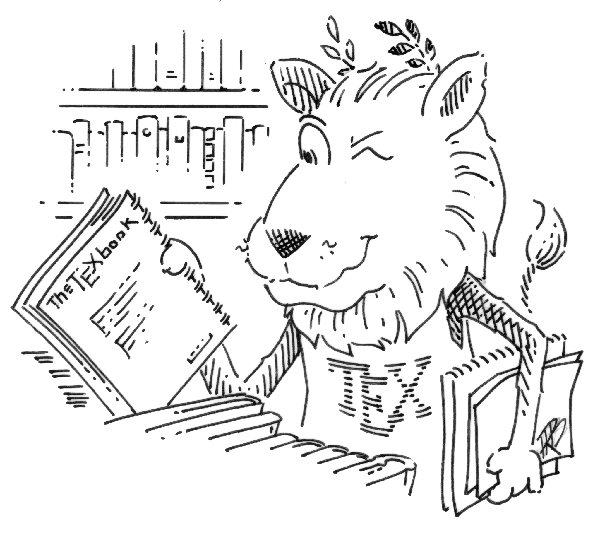
\includegraphics[trim=0cm 4cm 6cm 0cm, clip=true, width=7cm, angle=34]{figures/loewe.png}
\caption{Der \LaTeX-Löwe}
\label{fig:loewe}
\end{figure}

\ref{fig:loewe}
\mysideref{loewe}



%--
% Verweise auf Abbildungen bitte in den Seitenrand.
%--


Wilhelm von Humboldt

\begin{figure}
\includegraphics[width=0.4\textwidth]{wilhelm}
\caption{Wilhelmv von Humboldt (1767--1835)}
\label{fig:wilhelm}
\end{figure}
% ---
% Hier bitte das Bild von Wilhelm vH einfügen
% Datei: wilhelm
% Bildunterschrift: Wilhelm von Humbolt (1767--1835)
% ---

Friedrich Wilhelm Christian Carl Ferdinand von Humboldt (* 22. Juni 1767 in Potsdam; † 8. April 1835 in Tegel) war ein preußischer Gelehrter, Schriftsteller und Staatsmann. Als Bildungsreformer initiierte er die Neuorganisation des Bildungswesens im Geiste des Neuhumanismus und betrieb die Gründung der Friedrich-Wilhelms-Universität Berlin.

Zusammen mit seinem Bruder Alexander von Humboldt zählt er zu den großen, fortwirkend einflussreichen Persönlichkeiten in der deutschen Kulturgeschichte. Während Alexander dabei vor allem der erd- und naturwissenschaftlichen Forschung neue Horizonte erschlossen hat, lagen die Schwerpunkte für Wilhelm in der Beschäftigung mit kulturwissenschaftlichen Zusammenhängen wie der Bildungsproblematik, der Staatstheorie, der analytischen Betrachtung von Sprache, Literatur und Kunst sowie in aktiver politischer Mitgestaltung als Reformmotor im Schul- und Universitätswesen und als preußischer Diplomat.

%--
% VERWEIS auf wilhelm
%--
Siehe \ref{fig:wilhelm}

Inmitten aller Vielfalt der von aufklärerischen Impulsen bestimmten, gemeinwohlorientierten Betätigungen in Politik, Bildungswesen, Kultur und Wissenschaft hatte Wilhelm von Humboldt stets zugleich die Auslotung und Bildung der eigenen Individualität und Persönlichkeit im Blick. In der wiederum auf menschliche Individuen allgemein anzuwendenden Zielformel geht es um „die höchste und proportionierlichste Ausbildung aller menschlichen Kräfte zu einem Ganzen“.


Alexander von Humboldt
Friedrich Wilhelm Heinrich Alexander von Humboldt (* 14. September 1769 in Berlin; † 6. Mai 1859 ebenda) war ein deutscher Naturforscher mit einem weit über Europa hinausreichenden Wirkungsfeld. In seinem über einen Zeitraum von mehr als sieben Jahrzehnten entstandenen Gesamtwerk schuf er „einen neuen Wissens- und Reflexionsstand des Wissens von der Welt“[1] und wurde zum Mitbegründer der Geographie als empirischer Wissenschaft. Er war der jüngere Bruder von Wilhelm von Humboldt.

Seine mehrjährigen Forschungsreisen führten ihn nach Lateinamerika, in die USA sowie nach Zentralasien. Wissenschaftliche Feldstudien betrieb er unter anderem in den Bereichen Physik, Chemie, Geologie, Mineralogie, Vulkanologie, Botanik, Vegetationsgeographie, Zoologie, Klimatologie, Ozeanographie und Astronomie, aber auch zu Fragen der Wirtschaftsgeographie, der Ethnologie und der Demographie. Zudem korrespondierte er bei seinem publizistischen Werk mit zahlreichen international bedeutenden Spezialisten der verschiedenen Fachrichtungen und schuf so ein wissenschaftliches Netzwerk eigener Prägung.
%--
% VERWEIS auf alexander 
%--
Siehe \ref{fig:alexander}

In Deutschland erlangte er vor allem mit den Ansichten der Natur und dem Kosmos außerordentliche Popularität. Sein bereits zu Lebzeiten hohes Ansehen spiegelt sich in Bezeichnungen wie „der zweite Kolumbus“, „wissenschaftlicher Wiederentdecker Amerikas“, „Wissenschaftsfürst“ und „der neue Aristoteles“ (Gedenkmünze der Pariser Akademie der Wissenschaften). Er wurde in zahlreiche in- und ausländische Akademien aufgenommen.

\begin{figure}
\includegraphics[width=0.4\linewidth]{alexander}
\caption{Alexander von Humboldt (1769--1859)}
\label{fig:alexander}
\end{figure}
% ---
% Hier bitte das Bild von Alexander vH einfügen
% Datei: alexander
% Bildunterschrift: Alexander von Humbolt (1769--1859)
% ---


%---
% Wie kann man die Kompiliergeschwindigkeit erhöhen?
% Kann ich die Abbildungen auch (teilweise) ausblenden?
% Kann ich auch einen „Platzhalter-Text“ anstatt des Bildes setzen?
%---




\section{Abbildungen beschriften}
%---
% Kann ich auch noch eine Beschriftung in das Bild von Wilhelm bekommen?
% Vielleicht sowas wie „LaTeX ist toll!“
% Kannst du auch noch das Bild von Alexander in das Bild von Wilhelm integrieren?
%---
\section{Ausschnitthafte Vergrößerungen bei Abbildungen}

%---
% Das Bild von Wilhelm ist ja schön und gut, 
% aber ich kann sein Abzeichen nicht richtig erkennen.
% Kannst du dieses vergrößern?
%---



% !TEX root=../august-boeckh-hauptdokument.tex

\chapter[Kondizionale Operatoren]{Konditionale Operatoren. Das sind Boole’sche Operatoren, die eine Menge Spaß machen}

\section{Widmung}
%\toggletrue{hund}
Diese Doktorarbeit widme ich von Herzen 
\iftoggle{hund}
{meinem Hund.}
{meinen lieben Eltern.}

%---
%  Folgendes Szenario: In der offiziellen Abgabeversion möchte ich meinen Eltern danken. 
%  Aber ein Extraexemplar soll meinem Hund gewidmet sein.
% Kann man das machen, dass man das irgendwie automatisch ändern kann?
%---


\section{Abbildungen}




\begin{figure}[h]
{\missingcopyright%muss in geschweifte Klammern gesetzt werden, da Schalter
\subcaptionbox%
{Alexander von Humboldt}%
{\includegraphics[
height=0.4\textwidth]{figures/alexander.jpg}}}
\hfill
\subcaptionbox{Wilhelm von Humboldt}{\includegraphics[height=0.4\textwidth]{figures/wilhelm.jpg}}
\label{fig:bruederhumboldt}
\caption{Die zwei Brüder von Humboldt}
\end{figure}



%--------------------------------
% Jetzt wird es schwierig: Die zwei Brüder sollen nebeneinander gesetzt werden.
% alexander.jpg und wilhelm.jpg
% Als Bildunterschrift: Alexander von Humboldt // Wilhelm von Humboldt
% Als gemeinsame  Bildunterschrift: Die Brüder von Humboldt
% Die Bilder bitte gleich hoch setzen.
%-------------------------------


%---
% Ich habe allerdings nur für Wilhelm die Druckgenehmigung bekommen,
% nicht für Alexander.
% Das heißt, dass in meiner Abgabeversion beide Bilder zusehen sein müssen,
% in der finalen Printfassung muss Alexander ausgeblendet werden.
% Die Maße und die Bildunterschrift sollen erhalten bleiben
% und nur das Bild mit einem Platzhaltertext versehen werden.
%---








% !TEX root=../august-boeckh-hauptdokument.tex

\chapter{Tafelabbildungen}

% --
% Ans Ende der Arbeit kommt ein Tafelteil, Nummerierung als Taf. X, jede Seite wieder neu beginnen.
%--


\appendix%ändert die Nummerierung
% !TEX root=../august-boeckh-hauptdokument.tex

\chapter{Katalog der Häuser}

Hier kommt nun mein Katalog.
\renewcommand\thesection{Kat.\arabic{section}}

\DTLforeach{haeuser}%
{\house=house,%
\mylabel=label,%
\size=size,%
\mydescription=description,%
\location=location,%
\interior=interior,%
\interiorM=interiorM,%
\interiorW=interiorW,%
\interiorS=interiorS}%
{\section{\house}
\label{cat:\mylabel}
\mydescription
\begin{labeling}{Ausstattung}
	\item[Größe] \size\thinspace\square\meter%Befehl zum Aufrufen von SI-Einheiten, typographisch korrekt.
	\item[Ort] \location
	\item[Ausstattung]\ifdefempty{\interior}{~}{\interior}%Fake-Leerzeichen wegen direkt anschließender neuer Umgebung.
	\begin{description}
		\item[Mosaiken] \interiorM
		\item[Wandgemälde] \interiorW
		\ifdefempty{\interiorS}{}{
		\item[Skulptur] \interiorS}
	\end{description}
\end{labeling}%
}


Schön ist das Haus \ref{cat:M-Fabius-Rufus}.

}%false (testdokument)


\end{document}